
\begin{frame}
    \frametitle{State of the Field}
    \begin{columns}
        \begin{column}{0.65\textwidth}
            \textit{Active areas of research include:} \\ ~ \\
            % \uncover<1->{\alert{Global coverage to observe large-scale atmospheric dynamics}
            %     \begin{itemize}
            %         \footnotesize
            %         \item[$\blacktriangleright$] More observations over a larger area  
            %     \end{itemize}}
                
            \uncover<1->{\alert{Better analytical methods}
            \begin{itemize}
                \footnotesize
                \item[$\blacktriangleright$] Many ways to combine observations for analysis
                \item[$\blacktriangleright$] Numerous atmospheric phenomena to study
                \item[$\blacktriangleright$] Dense networks enable new analytical techniques
                \item[$\blacktriangleright$] Finer temporal and spatial resolution
            \end{itemize}}

            \uncover<2->{\alert{Multi-instrument analysis}
            \begin{itemize}
                \footnotesize
                \item[$\blacktriangleright$] Combining observations from many meteor radars
                \item[$\blacktriangleright$] Utilizing meteor radar with other atmospheric instruments
                \item[$\blacktriangleright$] Integrating into global circulation models
            \end{itemize}}

            \uncover<3->{\alert{Continued instrumentation development}
            \begin{itemize}
                \footnotesize
                \item[$\blacktriangleright$] Cheaper instruments for wider deployments 
                \item[$\blacktriangleright$] More capable instruments for better observations 
                \item[$\blacktriangleright$] Purposeful design of optimal radar networks 
            \end{itemize}}
        \end{column}
        \begin{column}{0.45\textwidth}%
            \centering%
            \noindent
            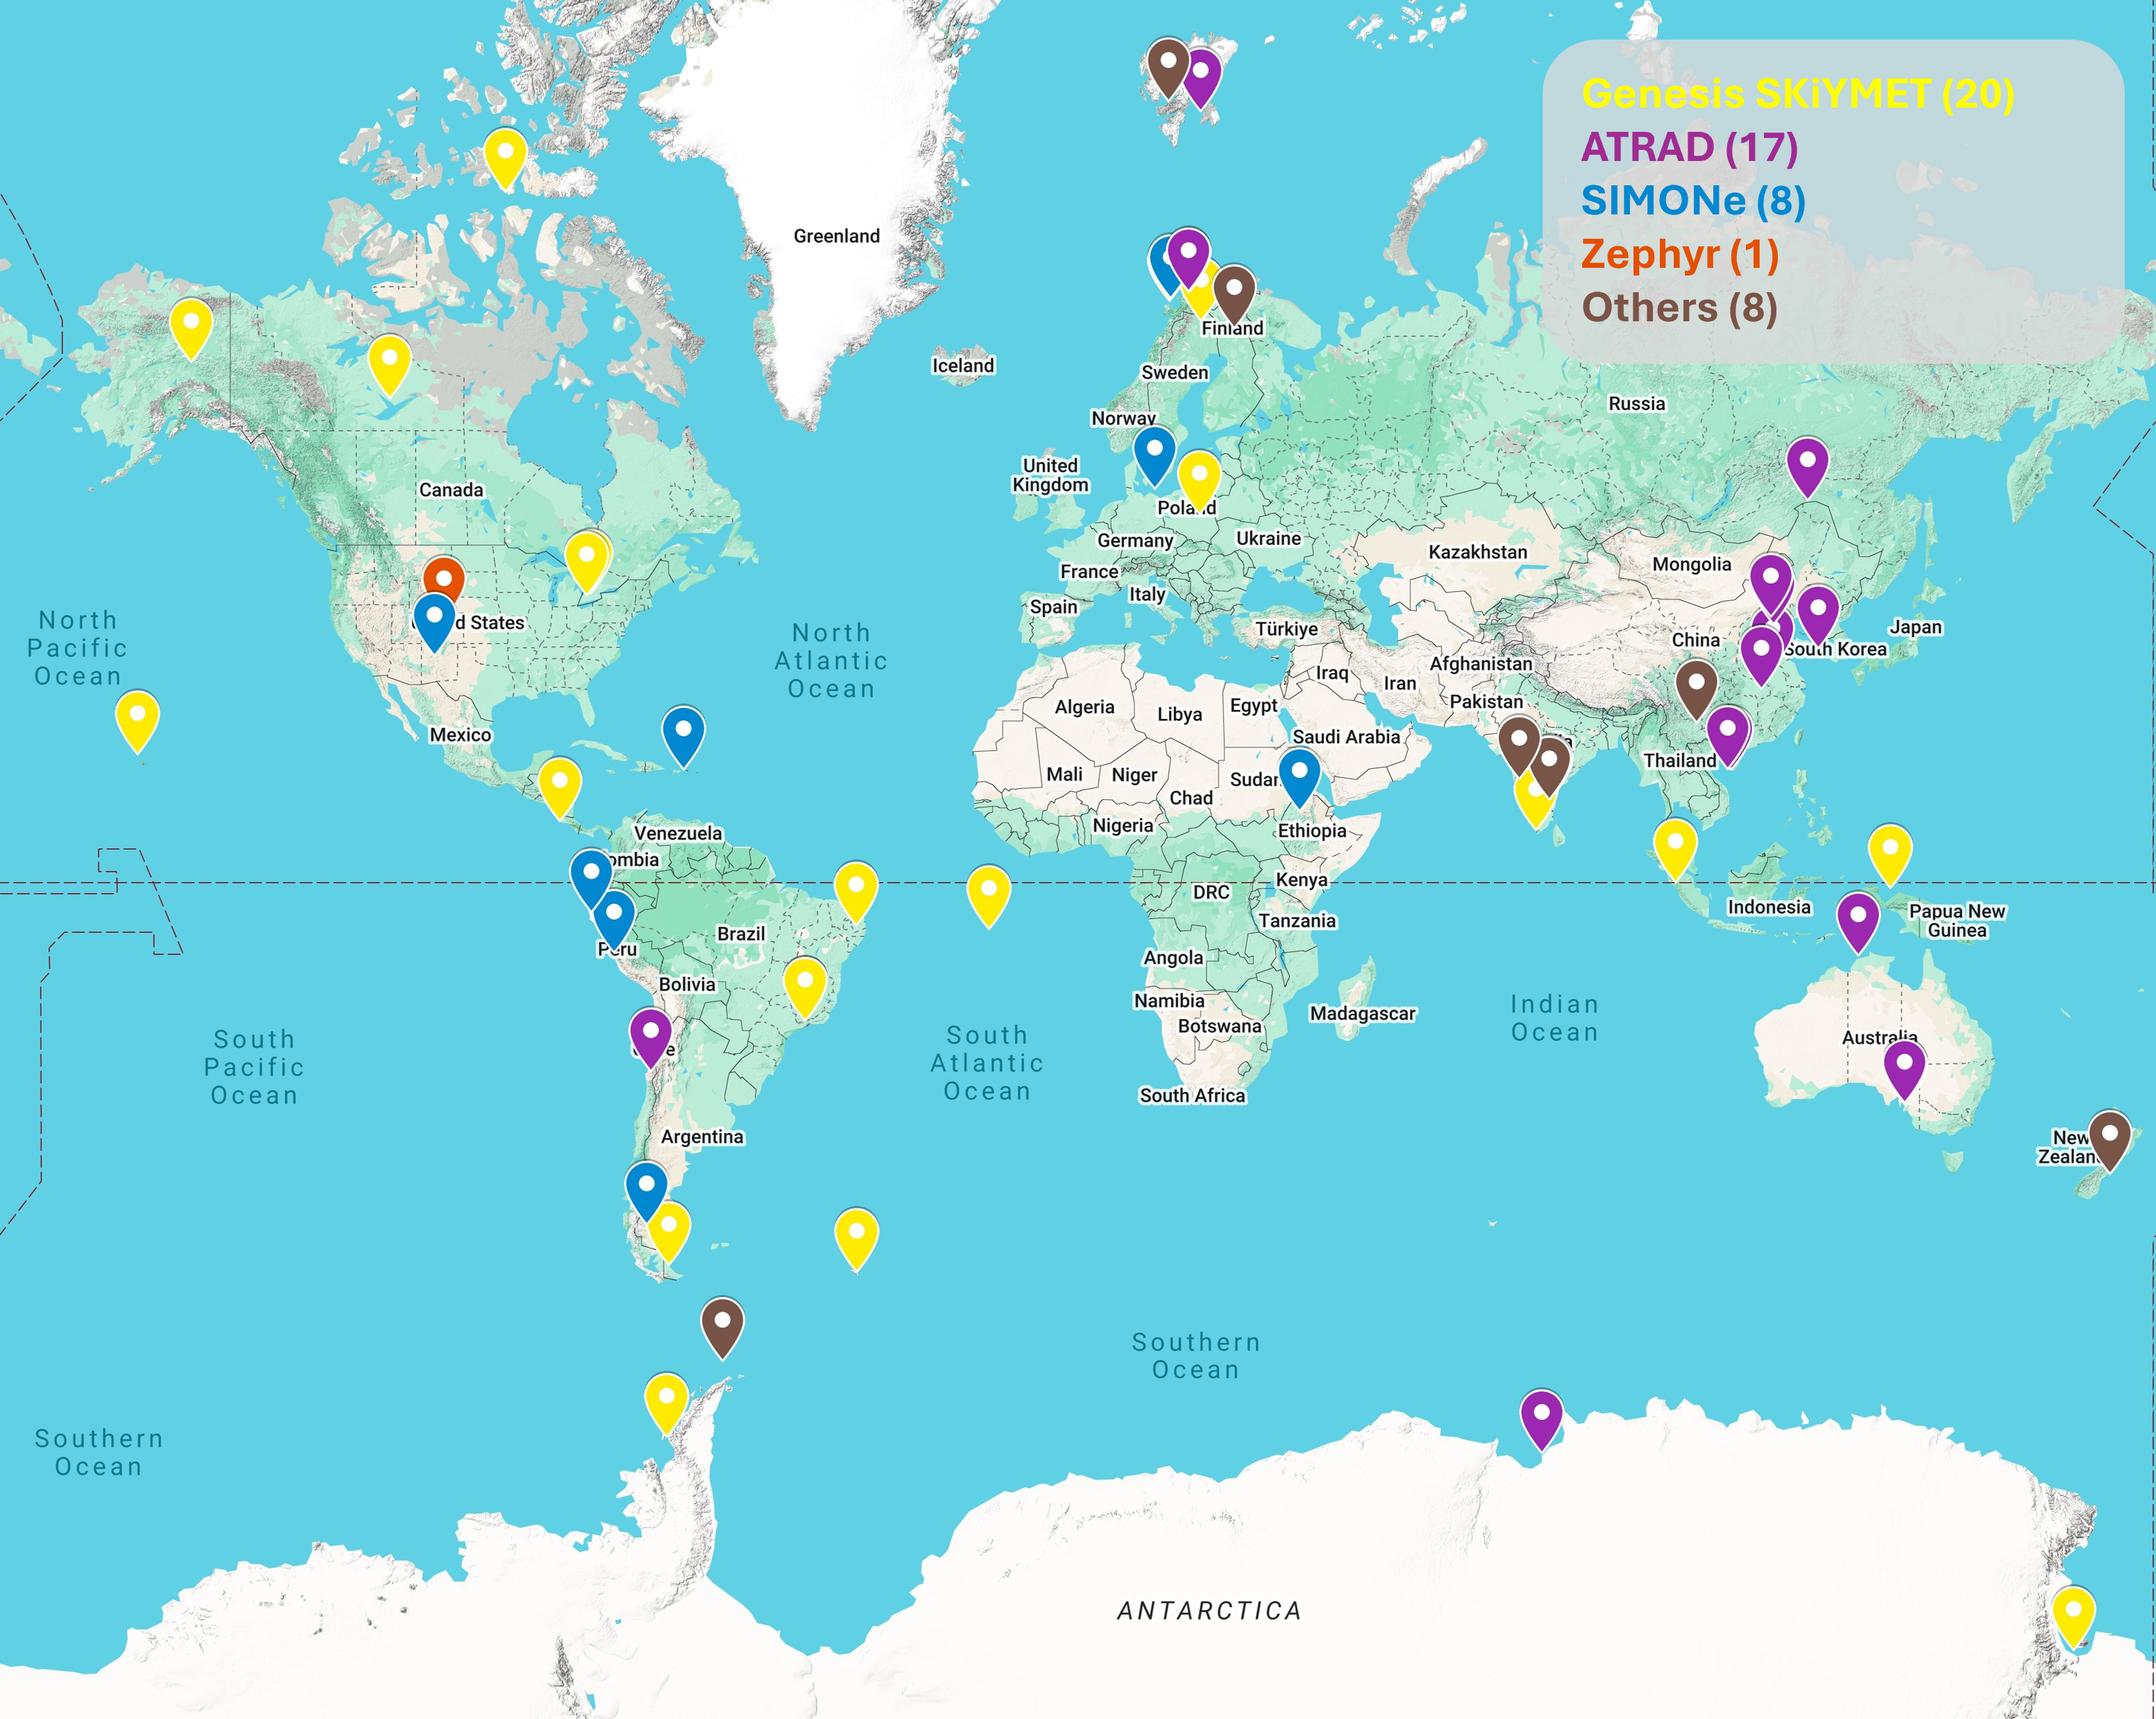
\includegraphics[width=\linewidth]{img/smr_map.png}
            \footnotesize
            \textit{Map of Contemporary Meteor Radars}
        \end{column}
    \end{columns}
\end{frame}